\documentclass{ximera}

\newcommand{\dfn}{\textbf}
\renewcommand{\vec}[1]{{\overset{\boldsymbol{\rightharpoonup}}{\mathbf{#1}}}\hspace{0in}}
%% Simple horiz vectors
\renewcommand{\vector}[1]{\left\langle #1\right\rangle}
\newcommand{\arrowvec}[1]{{\overset{\rightharpoonup}{#1}}}
\newcommand{\R}{\mathbb{R}}
\newcommand{\transpose}{\intercal}
\newcommand{\ro}{\texttt{R}}%% row operation
\newcommand{\dotp}{\bullet}%% dot product

\usetikzlibrary{calc,bending}
\tikzset{>=stealth}


\usepackage{mdframed} % For framing content
%\usepackage{ifthen}   % For conditional statements

% Define the 'concept' environment with an optional header
\newenvironment{concept}[1][]{%
  \begin{mdframed}[linecolor=black, linewidth=2pt, innertopmargin=5pt, innerbottommargin=5pt, skipabove=12pt, skipbelow=12pt]%
    \noindent\large\textbf{#1}\normalsize%
}{%
  \end{mdframed}%
}











%% \colorlet{textColor}{black}
%% \colorlet{background}{white}
%% \colorlet{penColor}{blue!50!black} % Color of a curve in a plot
%% \colorlet{penColor2}{red!50!black}% Color of a curve in a plot
%% \colorlet{penColor3}{red!50!blue} % Color of a curve in a plot
%% \colorlet{penColor4}{green!50!black} % Color of a curve in a plot
%% \colorlet{penColor5}{orange!80!black} % Color of a curve in a plot
%% \colorlet{penColor6}{yellow!70!black} % Color of a curve in a plot
%% \colorlet{fill1}{penColor!20} % Color of fill in a plot
%% \colorlet{fill2}{penColor2!20} % Color of fill in a plot
%% \colorlet{fillp}{fill1} % Color of positive area
%% \colorlet{filln}{penColor2!20} % Color of negative area
%% \colorlet{fill3}{penColor3!20} % Fill
%% \colorlet{fill4}{penColor4!20} % Fill
%% \colorlet{fill5}{penColor5!20} % Fill
%% \colorlet{gridColor}{gray!50} % Color of grid in a plot


\author{Bart Snapp}
%%OpenAI. (2023). ChatGPT (Mar 14 version) [Large language model]. https://chat.openai.com/chat

\title{Vectors, scalars, and matrices}


\begin{document}
\begin{abstract}
  A concrete introduction to vectors and matrices, with an informal
  view towards vector spaces and linear transformations.
\end{abstract}
\maketitle


\section{Vectors and scalars}

In mathematics, we study (among other things) numbers. In many cases,
these numbers represent real-world data. Sometimes it ``makes sense''
to add data and sometimes it doesn't.
\begin{concept}[When it does NOT make sense to add data]
\begin{description}
\item[Personal Identification Numbers] Summing things like social
  security numbers, phone numbers, or zip codes doesn't provide
  meaningful information.
\item[Temperatures] While you can mathematically add temperatures
  together, doing so usually doesn't provide useful information.
\item[Time] Adding specific points in time, like dates or hours of the
  day, usually doesn't yield meaningful results.
\item[Geographic Coordinates] Adding the latitude and longitude of two
  locations doesn't give you a location that has any real-world
  significance.
\end{description}
\end{concept}
For some of the categories above, the \textit{average} can be
meaningful; or perhaps if each quantity is thought of as
`displacement' or `duration,' summing might be meaningful. However,
without additional (pun intended!) stipulations, summing the types of
quantities above is not meaningful. On the other hand, there's lots of
times that it makes sense to add data:

\begin{concept}[When it makes sense to add data]
\begin{description}
\item[Population Counts] Adding the populations of different regions,
  cities, or countries to find the total population of a larger
  area. Answers to questions like these help us understand our
  society and are important to many people.
\item[Financial Transactions] Summing daily sales to find total
  monthly sales, or adding up all expenses to find total costs. These
  are real numbers that represent actual amounts of money, and their
  total gives meaningful information about financial status or
  performance.
\item[Time Spent on Tasks] Adding the duration of time spent on
  various activities on day gives a total time spent. We all have busy
  lives, and time is a very precious commodity. Hence, it is good to
  understand how we spend our time.
\item[Navigation] Aircraft navigate by knowing the direction and speed
  that they are traveling. When interpreted correctly, we add the
  speed and direction of many of many different ``course changes'' to
  find the ultimate position of the aircraft.
\end{description}
\end{concept}
Often when it make sense to \textit{add} quantities, it make sense to
\textit{scale} them as well. For example with population, you could
ask for the population of a city with $3$ times the population, or
half the population. Similar \textit{scaling} examples exist for all
the examples above where it make sense to add data. Regular old
numbers used to scale vectors are called \textit{scalars}.


\begin{definition}
  We say data is represented by \dfn{vectors} $\vec{v}$ and $\vec{w}$
  if
  \[
  \vec{v}+\vec{w}
  \]
  is also a vector, encoding `meaningful' data in the same way that
  $\vec{v}$ and $\vec{w}$ do, and for all \textbf{scalars} $s$, where
  $s$ is usually a real number,
  \[
  s(\vec{v} + \vec{w}) = s\vec{v}+ s\vec{w}.
  \]
  again represents `meaningful' data in the same way that $\vec{v}$
  and $\vec{w}$ do.
\end{definition}
These informal definitions of vectors and scalars in fact contain the
\textit{essence} of the concept of a \textit{vector space}. If this
seems too abstract, let's give some very concrete examples, based on
the examples above. However, before we start, we need to give some
notation for vectors.

\begin{concept}[Ways data can be stored as a vector]
\begin{description}
\item[As an ordered tuple] An ordered pair is just a pair of numbers
  $(a,b)$ delineated by parenthesis with the entries separated by a
  comma. It's called ``ordered'' because $(a,b) \ne (b,a)$. An \textit{ordered
  tuple} is just a list of an arbitrary, but fixed, number of elements
  that is ordered like an ordered pair. As an example, we could
  represent the \link[demographic information]{https://worldpopulationreview.com/states/states-by-race} for Ohio as an vector
  represented by an ordered tuple:
  \[
  \vec{p}_{\texttt{OH}} = (\underset{\text{White}}{9394878},\underset{\text{Black}}{1442655},\underset{\text{American Indian}}{20442},\underset{\text{Asian}}{268527},\underset{\text{Hawaiian}}{3907},\underset{\text{Other}}{544866})
  \]
\item[As a row vector] A row vector is a lot like an ordered tuple,
  except we do not use a comma to separate entries. Instead, we use a
  space.  Suppose a bookstore sells a variety of books in a month, say
  $141$ Science Fiction,
  $304$ Fantasy,
  $249$ Mystery,
  $199$ Romance,
  $251$ Historical.
  We can express this data as a row vector:
  \[
  \vec{s} = \begin{pmatrix}141 & 304 & 249 & 199 & 251 \end{pmatrix}
  \]
\item[As a column vector] A column vector is just like a row vector,
  except is it written vertically:
  \[
  \vec{w}_{\texttt{TR}} = \begin{pmatrix}
    0.5\\ 4 \\ 0 \\ 1\end{pmatrix}
    \qquad
    \begin{array}{l}
    \text{Emails}\\
    \text{Classes}\\
    \text{Projects}\\
    \text{Exercising}
  \end{array}
  \]
  Above, we could suppose that $\vec{w}_{\texttt{TR}}$ represents the
  fact that on Tuesdays and Thursdays, someone spends $0.5$ hours on
  emails, $4$ hours in class, $0$ hours on projects, and $1$ hour
  exercising.
\end{description}
\end{concept}

Of course, since mathematics is a human endeavor you will find variations on the notation above, as a common example, some folks use different brackets like these
\[
\langle a, b, c\rangle \qquad\text{or}\qquad
\begin{bmatrix}
  a\\
  b\\
  c
\end{bmatrix}
\]
for an ordered-tuple vectors and column vectors. Ordered tuples and
row vectors are more convient to write in a line, because they are
horizontal. On the other hand, column vectors take up less horizontal
space, and are more convenient when you have vectors with many entries.


\begin{definition}
  To switch a row vector into a column vector and vice versa, we use the \dfn{transpose} operation:
  \[
  \begin{pmatrix} 1 &  2 & 3 \end{pmatrix}^\transpose =
  \begin{pmatrix} 1 \\ 2 \\ 3 \end{pmatrix}
  \quad\text{and}\quad
  \begin{pmatrix} 1 \\ 2 \\ 3 \end{pmatrix}^\transpose =
  \begin{pmatrix} 1 &  2 & 3 \end{pmatrix}
  \]
\end{definition}


\begin{question}
  Consider $\vec{s} = \begin{pmatrix}141 & 304 & 249 & 199 & 251 \end{pmatrix}$. Compute $\vec{s}^\transpose$.
  \begin{prompt}
  \[
  \vec{s}^\transpose  = \begin{pmatrix}\answer{141} \\ \answer{304} \\ \answer{249} \\ \answer{199} \\ \answer{251} \end{pmatrix}
  \]
  \end{prompt}
\end{question}

Once we have data represented as vectors encoded as ordered tuples,
row vectors, or column vectors, we can describe some general
information about the vectors. In particular, we can think about their
\textit{dimension} and their \textit{components}.

\begin{definition}
The \dfn{dimension} of a vector is the number of entries. Each
individual entry of a vector is called a \dfn{component}.
\end{definition}

\begin{question}
  What is the dimension of the vector $\vec{p}_{\texttt{OH}}$?
  \begin{prompt}
  \[
  \text{Dimension} = \answer{6}
  \]
  \end{prompt}
\end{question}


When we express vectors as ordered tuples, row vectors, or column
vectors we add them in a componentwise fashion.
\begin{align*}
  (1,2,3) + (4,5,6) &= (5,7,9)\\
  \begin{pmatrix} 1 & 2 & 3   \end{pmatrix} + \begin{pmatrix} 4 & 5 & 6   \end{pmatrix} &= \begin{pmatrix} 5 & 7 & 9   \end{pmatrix}\\
  \begin{pmatrix} 1\\ 2\\ 3   \end{pmatrix} + \begin{pmatrix} 4\\ 5\\ 6   \end{pmatrix} &= \begin{pmatrix} 5\\ 7\\ 9   \end{pmatrix}
\end{align*}

We can also multiply vectors by a \dfn{scalar} (a number), by
multiplying each component by the scalar.
\begin{align*}
  5\cdot   (1,2,3) &= (5,10,15)\\
  5\cdot \begin{pmatrix} 1 & 2 & 3   \end{pmatrix}  &= \begin{pmatrix} 5 & 10 & 15   \end{pmatrix}\\
  5\cdot  \begin{pmatrix} 1\\ 2\\ 3   \end{pmatrix} &= \begin{pmatrix} 5\\ 10\\ 15   \end{pmatrix}
\end{align*}
Now that we know the basics, onto the examples!

\begin{example}[Population Counts] %https://worldpopulationreview.com/states/states-by-race
  The Midwest of the United States consists of $12$ states. We can
  express the $2023$
  \link[demographics]{https://worldpopulationreview.com/states/states-by-race}
  of each state as a vector represented by an ordered tuple. The
  ordered tuple for Ohio looks like:
  \[
  \vec{p}_{\texttt{OH}} = (\underset{\text{White}}{9394878},\underset{\text{Black}}{1442655},\underset{\text{American Indian}}{20442},\underset{\text{Asian}}{268527},\underset{\text{Hawaiian}}{3907},\underset{\text{Other}}{544866}).
  \]
  The ordered tuples for each state in the Midwest looks like:
\begin{align*}
  \vec{p}_{\texttt{IA}} &= (2806418,117035,10538,79296,3941,132783)\\
  \vec{p}_{\texttt{IL}} &= (8874067,1796660,33972,709567,5196,1296702)\\
  \vec{p}_{\texttt{IN}} &= (5510354,631923,14030,158705,2205,379676)\\
  \vec{p}_{\texttt{KA}} &= (2416165,165837,22278,87093,2344,218902)\\
  \vec{p}_{\texttt{MI}} &= (7735902,1360149,50035,316844,3117,507860)\\
  \vec{p}_{\texttt{MN}} &= (4572149,359817,54558,275242,2201,336199)\\
  \vec{p}_{\texttt{MO}} &= (4978046,698043,24274,123810,8887,291100)\\
  \vec{p}_{\texttt{ND}} &= (651470,23959,39165,11979,1004,32817)\\
  \vec{p}_{\texttt{NE}} &= (1641256,91896,16875,47944,1235,124620)\\
  \vec{p}_{\texttt{OH}} &= (9394878,1442655,20442,268527,3907,544866)\\
  \vec{p}_{\texttt{SD}} &= (735228,18836,74975,12413,544,37340)\\
  \vec{p}_{\texttt{WI}} &= (4895065,367889,48674,163396,2672,329279)
\end{align*}
\begin{enumerate}
\item What are the combined demographics of the states Michigan, Ohio,
  and Indiana?
\item Suppose that the annual percentage growth rate of Ohio is
  currently $0.1\%$. Assuming this is even across all demographics,
  what might the population data look like for Ohio in $2025$?
\end{enumerate}
\begin{solution}
  We'll use the properties of vectors to solve this problem.
  \begin{enumerate}
  \item To find the combined demographics of Michigan, Ohio, and
    Indiana we compute
    \[
    \vec{p}_{\texttt{MI}} + \vec{p}_{\texttt{OH}} + \vec{p}_{\texttt{IN}} = (\answer[given]{7735902+9394878+5510354},\answer[given]{},\answer[given]{},\answer[given]{},\answer[]{},\answer[given]{})
    \]
  \item To find the population growth of each demographic, we use the scalar, $1.001$ to find
    \[
    1.001 \vec{p}_{\texttt{OH}} =
    \]
  \end{enumerate}
\end{solution}
\end{example}



\begin{example}[Financial Transactions]
  A bookstore sells a variety of books. We'll express the number of
  each type of book sold in one month as a row vector
  \[
  \vec{s} = \begin{pmatrix}141 & 304 & 249 & 199 & 251 \end{pmatrix}
  \]
  with the entries representing the categories: Science Fiction,
  Fantasy, Mystery, Romance, Historical in that order.  If each book
  costs the bookstore $6$ dollars from the wholesaler, and each book sells
  for $9$ dollars, what is the profit for each category?
  \begin{solution}
    Using the properties of vectors, we wish to compute
    \[
    9\vec{s}-6\vec{s} =
    \]
  \end{solution}

\end{example}



\begin{example}[Time Spent on Tasks]
  On Mondays, Wednesdays, and Fridays, suppose you spend you spend $1$
  hour on emails, $2$ hours in class, and $3$ hours working on
  projects. On Tuesdays and Thursdays, you spend $1/2$ hour on emails,
  $4$ hours in class, and $1$ hour exercising. We can express each day
  as a column vector:
  \[
  \vec{w}_{\texttt{MWF}} =
  \begin{pmatrix}
    1 \\
    2 \\
    3 \\
    0
  \end{pmatrix}
  \qquad
  \vec{w}_{\texttt{TR}} =
  \begin{pmatrix}
    0.5\\
    4\\
    0\\
    1
  \end{pmatrix} \qquad
  \begin{array}{l}
    \text{Emails}\\
    \text{Classes}\\
    \text{Projects}\\
    \text{Exercising}
  \end{array}
  \]
  How much time is spent on emails, classes, projects, and exercising
  per work week?
  \begin{solution}
    Here we simply compute:
    \[
    3 \vec{w}_{\texttt{MWF}} + 2  \vec{w}_{\texttt{TR}}  =
    \]
  \end{solution}
\end{example}




\begin{example}[Navigation]
  Airplanes can use true bearings for navigation. Here's the idea, the direction is given by degrees from North:

\begin{center}
\upshape
% Define a few constants for easy configuration
\def\radius{2cm}
\def\onedegrad{1.8cm}
\def\fivedegrad{1.75cm}
\def\tendegrad{1.7cm}
\def\labelrad{1.6cm}

\begin{tikzpicture}[scale=1.3] %% https://texample.net/tikz/examples/degree-wheel/
  \draw[ultra thick] (0,0) circle (\radius);
  % labels and longer lines at every 10 degrees
  \node at (0,.65*\radius) {\bf N};
  \node at (0,-.65*\radius) {\bf S};
  \node at (-.65*\radius,0) {\bf W};
  \node at (.65*\radius,0) {\bf E};
  \foreach \x in {0,10,...,350}
  {
    \node[scale=.5, rotate=\x*-1] at (360-\x+90:\labelrad) {\x};
    \draw[thick] (\x:\tendegrad) -- (\x:\radius);
  };

  % lines at every 5 degrees
  \foreach \x in {0,5,...,355}  \draw (\x:\fivedegrad) -- (\x:\radius);

\end{tikzpicture}
\end{center}

So traveling North would be a (true) bearing of $0^\circ$, while
traveling West would be a bearing of $270^\circ$.
\link[knots]{https://en.wikipedia.org/wiki/Knot_(unit)}.
\begin{enumerate}
\item Suppose a plane starts at $(0,0)$ and its destination is reached
  by following true bearing $280^\circ$ for $3$ hours at $125$ knots.
  What are the coordinates of planes destination?
\item Suppose further there is wind blowing at $35$ knots in the true
  bearing of $110^\circ$. In this case, what are the coordinates of
  the plane after it has traveled on bearing $280^\circ$ at $125$
  knots for $3$ hours?
%% \item What course and speed should the pilot set to arrive at the
%%   destination on-time?
\end{enumerate}

\begin{solution}
While it makes sense (separately) to add speeds and angles, we cannot
directly make a vector from this information because there is no
obvious way to ``add'' ordered tuples of speed and angle. However, we
can convert a true bearing of $\beta$ along with a speed $v$ to
cartesian coordinates by writing:
\[
\begin{pmatrix}v\cdot \sin(\beta)\\ v \cdot \cos(\beta)\end{pmatrix}
\]
Armed with this, we are ready to solve the problem.
\begin{enumerate}
\item  Converting the planes bearing and speed to a vector in cartesian
  coordinates, we have
  \[
  \vec{p} = \begin{pmatrix}125\cdot \sin(280^\circ)\\ 125 \cdot \cos(280^\circ)\end{pmatrix}
  \]
  Here is a schematic drawing of what is happening:

  \begin{center}
    %% A schematic diagram showing a vector at a 330 degree angle with a
    %% vertical line, made in a clockwise fashion. The vectors' length is labeled 125
    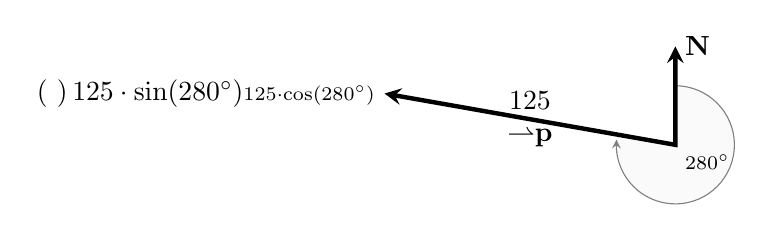
\begin{tikzpicture}[scale=2.5]
      \filldraw[fill=black!2!white,draw=none]
      (0,0) -- (0mm,3mm) arc (90:-190:3mm) -- (0,0);

      \draw[draw=white!50!black,->]
      (0mm,3mm) arc (90:-185:3mm);

      \draw[<->,ultra thick] ({1.5*sin(280)},{1.5*cos(280)}) -- (0,0) -- (0,.5);

      \node[below right] at (0,0) {$\scriptstyle 280^\circ$};
      \node[right] at (0,.5) {\bf N};
      \node[above]  at ({.75*sin(280)},{.75*cos(280)}) {$125$};
      \node[below]  at ({.75*sin(280)},{.75*cos(280)}) {$\vec{p}$};
      \node[left] at ({1.5*sin(280)},{1.5*cos(280)}) {$\begin{pmatrix}\scriptstyle 125\cdot \sin(280^\circ)\\ \scriptstyle 125 \cdot \cos(280^\circ)\end{pmatrix}$};
    \end{tikzpicture}
  \end{center}



To find the the coordinates of the plane after it has traveled for $3$
hours, we use $3$ as a scalar to write
\begin{align*}
  3\vec{p} &= \begin{pmatrix}\answer[given]{375}\cdot \sin(280^\circ)\\ \answer[given]{375} \cdot \cos(280^\circ)\end{pmatrix}\\
  &= \begin{pmatrix}\answer[given]{-369.30}\\ \answer[given]{65.12} \end{pmatrix}\\
\end{align*}
\item Now supposing that the wind blowing at $35$ knots in the true
  bearing of $110^\circ$, we have something like this:
  \begin{center}
    %% A schematic diagram showing a vector at a 330 degree angle with a
    %% vertical line, made in a clockwise fashion. The vectors' length is labeled 125
    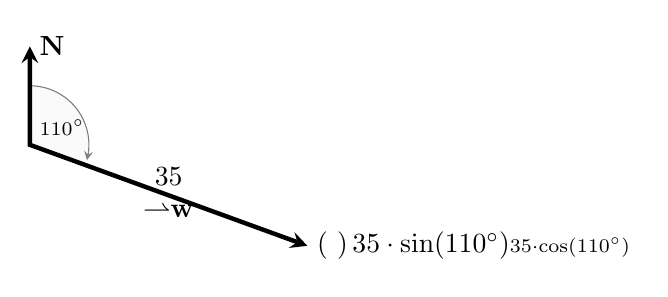
\begin{tikzpicture}[scale=2.5]
      \filldraw[fill=black!2!white,draw=none]
      (0,0) -- (0mm,3mm) arc (90:-20:3mm) -- (0,0);

      \draw[draw=white!50!black,->]
      (0mm,3mm) arc (90:-15:3mm);

      \draw[<->,ultra thick] ({1.5*sin(110)},{1.5*cos(110)}) -- (0,0) -- (0,.5);

      \node[above right] at (0,0) {$\scriptstyle 110^\circ$};
      \node[right] at (0,.5) {\bf N};
      \node[above]  at ({.75*sin(110)},{.75*cos(110)}) {$35$};
      \node[below]  at ({.75*sin(110)},{.75*cos(110)}) {$\vec w$};
      \node[right] at ({1.5*sin(110)},{1.5*cos(110)}) {$\begin{pmatrix}\scriptstyle 35\cdot \sin(110^\circ)\\ \scriptstyle 35 \cdot \cos(110^\circ)\end{pmatrix}$};

    \end{tikzpicture}
  \end{center}
  So now we can solve our problem by computing:
  \[
  3\vec{p} + 3 \vec{w} =
  \]
\end{enumerate}
\end{solution}
\end{example}



\section{Matrices store and transform data}


A \dfn{matrix} is just a big rectangular array of numbers
\[
M =
\underset{\displaystyle\boldsymbol{5}~\textbf{columns}}{\begin{pmatrix}
  a_{1,1} & a_{1,2} & a_{1,3} & a_{1,4} & a_{1,5} \\
  a_{2,1} & a_{2,2} & a_{2,3} & a_{2,4} & a_{2,5} \\
  a_{3,1} & a_{3,2} & a_{3,3} & a_{1,4} & a_{3,5} \\
  a_{4,1} & a_{4,2} & a_{4,3} & a_{4,4} & a_{4,5}
\end{pmatrix}}
\boldsymbol{4}~\textbf {rows}
\]
We give the \dfn{dimensions of a matrix} by stating its number of rows
and columns. Rows come first and columns come second, so $M$ above is
a $(4\times 5)$-matrix. We can use similar notation to talk about
specific entries of a matrix. Above, $a_{i,j}$ is the
$\boldsymbol{(i,j)}${\bf-}\dfn{entry} of the matrix $M$. Sometimes,
people write $M_{i,j}$ to mean the $(i,j)$-entry of the matrix $M$.

\begin{question}
  Which matrix below is a $3\times 2$ matrix?
  \[
  write more
  \]
\end{question}
In fact $n$-dimensional row vectors are just $1\times n$ matrices and
$n$-dimensional column vectors are just $n\times 1$ matrices.


\subsection{Matrices store data}


One way we get a matrix is by simply combining vectors. You can think
of a matrix a just a bunch of vectors stacked together.

\begin{example}[Population Counts] %https://worldpopulationreview.com/states/states-by-race
  In a previous example, we encoded the $2023$
  \link[demographics]{https://worldpopulationreview.com/states/states-by-race}~of
  the twelve Midwestern States as $6$-dimensional vectors, represented
  as an ordered tuples. Represent this data by a $12\times 6$
  matrix. Explain what the entry at position $(4,8)$ represents.
  \begin{solution}
  Since ordered-tuples are \wordChoice{\choice[correct]{horizontal}\choice{vertical}} it makes sense to
  concatenate this data by stacking it vertically into a matrix:
  \[
  \begin{pmatrix}
  \vec{p}_{\texttt{IA}} \\
  \vec{p}_{\texttt{IL}} \\
  \vec{p}_{\texttt{IN}} \\
  \vec{p}_{\texttt{KA}} \\
  \vec{p}_{\texttt{MI}} \\
  \vec{p}_{\texttt{MN}} \\
  \vec{p}_{\texttt{MO}} \\
  \vec{p}_{\texttt{ND}} \\
  \vec{p}_{\texttt{NE}} \\
  \vec{p}_{\texttt{OH}} \\
  \vec{p}_{\texttt{SD}} \\
  \vec{p}_{\texttt{WI}}
  \end{pmatrix}
  =
  \begin{pmatrix}
  2806418 & 117035 & 10538 & 79296 & 3941 & 132783\\
  8874067 & 1796660 & 33972 & 709567 & 5196 & 1296702\\
  5510354 & 631923 & 14030 & 158705 & 2205 & 379676\\
  2416165 & 165837 & 22278 & 87093 & 2344 & 218902\\
  7735902 & 1360149 & 50035 & 316844 & 3117 & 507860\\
  4572149 & 359817 & 54558 & 275242 & 2201 & 336199\\
  4978046 & 698043 & 24274 & 123810 & 8887 & 291100\\
  651470 & 23959 & 39165 & 11979 & 1004 & 32817\\
  1641256 & 91896 & 16875 & 47944 & 1235 & 124620\\
  9394878 & 1442655 & 20442 & 268527 & 3907 & 544866\\
  735228 & 18836 & 74975 & 12413 & 544 & 37340\\
  4895065 & 367889 & 48674 & 163396 & 2672 & 329279
  \end{pmatrix}
  \]
  The entry at position $(4,8)$ represents BADBAD
  \end{solution}
\end{example}

\begin{example}[Time Spent on Tasks]
  In a previous example, we encoded one's daily ``time spent on
  tasks'' for weekdays using $4$-dimensional vectors, represented as
  column vectors. Represent the five-day weekly ``time spent on task''
  by a $5\times 4$ matrix. Interpret the meaning of the $(2,3)$-entry
  of the matrix.
  \begin{solution}
    Since we are using column vectors, we'll concatenate this data by
    placing the vectors side-by-side:
    \[
    \begin{pmatrix}
      \vec{w}_{\texttt{MWF}} & \vec{w}_{\texttt{TR}} & \vec{w}_{\texttt{MWF}} & \vec{w}_{\texttt{TR}} & \vec{w}_{\texttt{MWF}}
    \end{pmatrix}
    =
    \begin{pmatrix}
      1 & 0.5 & 1 & 0.5 & 1 \\
      2 & 4   & 2 & 4   & 2 \\
      3 & 0   & 3 & 0   & 3 \\
      0 & 1   & 0 & 1   & 0
    \end{pmatrix}
    \]
    The meaning of the $(2,3)$-entry is BADBAD
  \end{solution}
\end{example}







\subsection{Multiplying vectors by matrices}

Baby-steps to multiplying matrices! We'll start by multiplying a $(1\times 3)$-matrix by a $(3\times 1)$ matrix
\[
\begin{pmatrix} a_{1,1} & a_{1,2} & a_{1,3} \end{pmatrix}
\begin{pmatrix} b_{1,1} \\ b_{2,1} \\ b_{3,1} \end{pmatrix} = a_{1,1}b_{1,1} + a_{1,2}b_{2,1} + a_{1,3}b_{3,1}
\]
This is equivalent to multiplying a row vector by a column vector. We
can imagine a `physical' movement of the entires with this product:

\begin{center}
  \begin{tikzpicture}
    \draw[line width=18pt, black!20!white, ->] (-.95,-.6) -- (-.95, .6) -- (-3,.6 );
    \node at (0,0) {\begin{minipage}{\textwidth}
        \begin{align*}
          \begin{pmatrix} a_{1,1} & a_{1,2} & a_{1,3} \end{pmatrix}
          \begin{pmatrix} b_{1,1} \\ b_{2,1} \\ b_{3,1} \end{pmatrix} &=
          \begin{pmatrix} a_{1,1} & a_{1,2} & a_{1,3} \end{pmatrix}\\
          &= a_{1,1}b_{1,1} + a_{1,2}b_{2,1} + a_{1,3}b_{3,1}
        \end{align*}
      \end{minipage}};
    \node at (1.5,.7) {$\begin{matrix} b_{1,1} & b_{1,2} & b_{1,3} \end{matrix}$};
  \end{tikzpicture}
\end{center}
We'll leave it to the reader to generalize this proceedure to $(1\times n)$-matrix by a $(n\times 1)$ matrix.

\begin{question}
  CHECK TO SEE IF THEY CAN GENERALIZE THE PROCEEDURE WITH n=4 and n=6 (use sparce matrices)
\end{question}


To multiply matrix by a column vector, envision the matrix as a
grouping of row vectors and we use the distributive property. for
example:
\begin{align*}
\begin{pmatrix}
  a_{1,1} & a_{1,2} & a_{1,3} \\
  a_{2,1} & a_{2,2} & a_{2,3} \\
  a_{3,1} & a_{3,2} & a_{3,3}
\end{pmatrix}
\begin{pmatrix} b_{1,1} \\ b_{2,1} \\ b_{3,1} \end{pmatrix}
&=
\begin{pmatrix}
  (a_{1,1} & a_{1,2} & a_{1,3}) \\
  (a_{2,1} & a_{2,2} & a_{2,3}) \\
  (a_{3,1} & a_{3,2} & a_{3,3})
\end{pmatrix}
\begin{pmatrix} b_{1,1} \\ b_{2,1} \\ b_{3,1} \end{pmatrix}\\
&=
\begin{pmatrix}
  (a_{1,1} & a_{1,2} & a_{1,3}) \begin{pmatrix} b_{1,1} \\ b_{2,1} \\ b_{3,1} \end{pmatrix}\\
  (a_{2,1} & a_{2,2} & a_{2,3}) \begin{pmatrix} b_{1,1} \\ b_{2,1} \\ b_{3,1} \end{pmatrix}\\
  (a_{3,1} & a_{3,2} & a_{3,3}) \begin{pmatrix} b_{1,1} \\ b_{2,1} \\ b_{3,1} \end{pmatrix}
\end{pmatrix}\\
&=
\begin{pmatrix}
  a_{1,1}b_{1,1} + a_{1,2}b_{2,1} + a_{1,3}b_{3,1}  \\
  a_{2,1}b_{1,1} + a_{2,2}b_{2,1} + a_{2,3}b_{3,1}  \\
  a_{3,1}b_{1,1} + a_{3,2}b_{2,1} + a_{3,3}b_{3,1}
\end{pmatrix}
\end{align*}

\begin{warning}
  It only makes sense to multiply a matrix by a column vector if the
  number of colmuns of the matrix equals the dimension of the column
  vector.
\end{warning}


In an entirely similar way, we can multiply a row vector by a matrix
by envisioning the matrix as a grouping of column vectors.



\begin{align*}
&\begin{pmatrix} a_{1,1} & a_{1,2} & a_{1,3} \end{pmatrix}
\begin{pmatrix}
  b_{1,1} & b_{1,2} & b_{1,3} \\
  b_{2,1} & b_{2,2} & b_{2,3} \\
  b_{3,1} & b_{3,2} & b_{3,3}
\end{pmatrix}
=
\begin{pmatrix} a_{1,1} & a_{1,2} & a_{1,3} \end{pmatrix}\arraycolsep=0pt
\begin{pmatrix}
  \begin{pmatrix} b_{1,1} \\ b_{2,1} \\ b_{3,1} \end{pmatrix} &
  \begin{pmatrix} b_{1,2} \\ b_{2,2} \\ b_{3,2} \end{pmatrix} &
  \begin{pmatrix} b_{1,3} \\ b_{2,3} \\ b_{3,3} \end{pmatrix}
\end{pmatrix} \\
&=\arraycolsep=0pt
\begin{pmatrix}
  \begin{pmatrix} a_{1,1} & a_{1,2} & a_{1,3} \end{pmatrix}\begin{pmatrix} b_{1,1} \\ b_{2,1} \\ b_{3,1} \end{pmatrix} &
  \begin{pmatrix} a_{1,1} & a_{1,2} & a_{1,3} \end{pmatrix}\begin{pmatrix} b_{1,2} \\ b_{2,2} \\ b_{3,2} \end{pmatrix} &
  \begin{pmatrix} a_{1,1} & a_{1,2} & a_{1,3} \end{pmatrix}\begin{pmatrix} b_{1,3} \\ b_{2,3} \\ b_{3,3} \end{pmatrix}
\end{pmatrix}\\
&=\arraycolsep=0pt
\begin{pmatrix}
a_{1,1}b_{1,1}+a_{1,2}b_{2,1}+a_{1,3}b_{3,1} &
a_{1,1}b_{1,2}+a_{1,2}b_{2,2}+a_{1,3}b_{3,2} &
a_{1,1}b_{1,3}+a_{1,2}b_{2,3}+a_{1,3}b_{3,3}
\end{pmatrix}
\end{align*}



\begin{warning}
  It only makes sense to multiply a row vector by a matrix if the
  dimension of the row vector equals the the number of rows of the
  matrix.
\end{warning}

\begin{example}[Population Counts]
Extract a new data set from a matrix using basis vectors
\end{example}


\begin{example}[Time Spent on Tasks]
\end{example}



\subsection{Matrices transform data}


\begin{example}[Financial Transactions]
  Recall that a bookstore sells a variety of books with each type of
  book sold in one month stored as a row vector
  \[
  \vec{s} = \begin{pmatrix}141 & 304 & 249 & 199 & 251 \end{pmatrix}
  \]
  with the entries representing the categories: Science Fiction,
  Fantasy, Mystery, Romance, Historical in that order.  Suppose last
  month the book store bought $200$ Science Fiction, $400$ Fantasy, $300$
  Mystery, $250$ Romance, $300$ Historical books. What percentage of each
  category was sold this month?
  \begin{solution}
    Let
    \[
    T =
    \begin{pmatrix}
      100/200 & 0 &    0   &   0    &   0 \\
      0 & 100/400 &    0   &   0    &   0 \\
      0 &   0   &  100/300 &   0    &   0 \\
      0 &   0   &    0   & 100/250  &   0 \\
      0 &   0   &    0   &   0    & 100/300
    \end{pmatrix}
    \]
    Each entry of the matrix $T$ is of the form:
    \[
    100 \cdot \frac{1}{(\text{Stock})}
    \]
    where $(\text{Stock})$ represents the number of books the
    bookstore bought to sell.  We can solve our problem by computing
    \[
    \vec{s} T =
    \]
    So we see
  \end{solution}

\end{example}




\begin{example}[Navigation]
  Scale/normalize fincinal data etc.
\end{example}







\end{document}
